%  Plantilla de trabajo recepcional - Tesis con formato artículo
%  Formato APA 7a edición
%  Universidad Juárez Autónoma de Tabasco (UJAT)
%
%  Motor pdflatex (compatible con distribuciones LaTeX antiguas).
%  Bibliografía con BibTeX + apacite.
%
%  Orden de compilación:
%     1) pdflatex main
%     2) bibtex   main
%     3) pdflatex main
%     4) pdflatex main
\documentclass[12pt,letterpaper]{report}

% ---------------------------------------------------------------
% 1. Configuración de idioma
% ---------------------------------------------------------------
\usepackage[utf8]{inputenc}
\usepackage[T1]{fontenc}
\usepackage[spanish,es-noindentfirst]{babel}
\AtBeginDocument{\selectlanguage{spanish}}

% ---------------------------------------------------------------
% 2. Configuración de página APA 7: 2.54 cm (1 in) en los cuatro lados
% ---------------------------------------------------------------
\usepackage{geometry}
\geometry{letterpaper, margin=2.54cm}

% ---------------------------------------------------------------
% 3. Configuración de tipografía: Arial 12 pt
% ---------------------------------------------------------------
\usepackage{helvet}
\renewcommand{\familydefault}{\sfdefault}


% ---------------------------------------------------------------
% 4. Paquetes útiles
% ---------------------------------------------------------------
\usepackage{graphicx}
\usepackage{indentfirst}
\usepackage{titlesec}
\usepackage{enumitem}
\usepackage{caption}
\usepackage{array}
\usepackage{longtable}
\usepackage{booktabs}
\usepackage{fancyhdr}
\usepackage{hyperref}
\usepackage{eso-pic}    % Imagen de fondo
\usepackage{soul}       % Resaltado de texto. Eliminar

% ---------------------------------------------------------------
% 6. Configuración de referencias: BibTeX + apacite (español, con DOI)
%    apacite debe cargarse después de hyperref.
% ---------------------------------------------------------------
\usepackage[doi,tocbib]{apacite}
% APA 7 exige que el DOI se muestre como URL completa (https://doi.org/...),
% en lugar del prefijo "doi:" que usa apacite por defecto.
\renewcommand{\doiprefix}{https://doi.org/\ignorespaces}

% ---------------------------------------------------------------
% 7. Configuración de índices
% ---------------------------------------------------------------
\addto\captionsspanish{%
  \renewcommand{\contentsname}{Índice de Contenido}%
  \renewcommand{\listtablename}{Índice de Tablas}%
  \renewcommand{\listfigurename}{Índice de Figuras}%
  \renewcommand{\tablename}{Tabla}%
  \renewcommand{\figurename}{Figura}%
  \renewcommand{\refname}{Referencias}%
  \renewcommand{\bibname}{Referencias}%
}

% ---------------------------------------------------------------
% 8. Configuración de contenido APA 7
% ---------------------------------------------------------------
\usepackage{setspace}  % Doble espacio
\doublespacing

\providecommand{\chaptername}{}  % Capítulos numerados en romano
\renewcommand{\chaptername}{Capítulo}

\setcounter{secnumdepth}{0}   % Ningún encabezado interno se numera
\setcounter{tocdepth}{1}      % El índice muestra el capítulo + 2 niveles

% Nivel 1: Capítulo: centrado, negrita, salto de página antes.
\titleformat{\chapter}[display]
  {\centering\bfseries\fontsize{16}{19}\selectfont}
  {}
  {0pt}
  {\centering\bfseries\fontsize{16}{19}\selectfont}
\titlespacing*{\chapter}{0pt}{0pt}{24pt}
% Comando \capitulo{Título}: crea un capítulo con salto de página
\newcounter{capitulo}
\renewcommand{\thecapitulo}{\Roman{capitulo}}
\newcommand{\capitulo}[1]{%
  \refstepcounter{capitulo}%
  \chapter*{\chaptername\ \thecapitulo. #1}%
  \addcontentsline{toc}{chapter}{\chaptername\ \thecapitulo. #1}%
}

% Nivel 2: Sección: alineado a la izquierda, negrita
\titleformat{\section}
  {\normalfont\bfseries}{}{0pt}{}
\titlespacing*{\section}{0pt}{18pt}{6pt}

% Nivel 3: Subsección: alineado a la izquierda, negrita cursiva
\titleformat{\subsection}
  {\normalfont\bfseries\itshape}{}{0pt}{}
\titlespacing*{\subsection}{0pt}{16pt}{6pt}

% Nivel 4: Subsubsección con sangría
\titleformat{\subsubsection}[runin]
  {\normalfont\bfseries}{}{0pt}{}[.]
\titlespacing*{\subsubsection}{1.27cm}{14pt}{1em}

% Nivel 5: Párrafo con sangría
\titleformat{\paragraph}[runin]
  {\normalfont\bfseries\itshape}{}{0pt}{}[.]
\titlespacing*{\paragraph}{1.27cm}{12pt}{1em}

% ---------------------------------------------------------------
% 9. Configuración de tablas y figuras
% ---------------------------------------------------------------
\DeclareCaptionLabelFormat{apaLabel}{#1 #2}
\captionsetup[table]{
  labelformat=apaLabel, labelsep=newline,
  justification=raggedright, singlelinecheck=false,
  font=singlespacing, labelfont=bf, textfont=it,
  position=top
}
\captionsetup[figure]{
  labelformat=apaLabel, labelsep=newline,
  justification=raggedright, singlelinecheck=false,
  font=singlespacing, labelfont=bf, textfont=it,
  position=top
}
% Nota al pie de tabla/figura
\newcommand{\apanota}[1]{%
  \par\vspace{4pt}\noindent\footnotesize\singlespacing
  \textit{Nota.} #1\par
}

% ---------------------------------------------------------------
% 10. Configuración del encabezado de página
% ---------------------------------------------------------------
\setlength{\headheight}{14.5pt}
\pagestyle{fancy}
\fancyhf{}
\fancyhead[R]{\thepage}
\renewcommand{\headrulewidth}{0pt}
\fancypagestyle{plain}{%
  \fancyhf{}
  \fancyhead[R]{\thepage}
  \renewcommand{\headrulewidth}{0pt}
}

% ---------------------------------------------------------------
% 11. Datos del trabajo recepcional
% ---------------------------------------------------------------
\newcommand{\tituloTrabajo}{[\hl{TÍTULO DEL TRABAJO RECEPCIONAL}]}
\newcommand{\gradoObtener}{[\hl{INGENIERO o INGENIERA EN SISTEMAS COMPUTACIONALES}]}
\newcommand{\tipoTrabajo}{TESIS PARA OBTENER EL GRADO DE:}
\newcommand{\nombreEstudiante}{[\hl{NOMBRE DEL ESTUDIANTE}]}
\newcommand{\nombreDirector}{[\hl{NOMBRE DEL PROFESOR(A)}]}
\newcommand{\lugarFecha}{CUNDUACÁN, TABASCO, A: [\hl{MES}] [\hl{AÑO}]}

\begin{document}

% Portada
\begin{titlepage}

\thispagestyle{empty}

\AddToShipoutPictureBG*{
  \AtPageUpperLeft{%
    \raisebox{-\height}{
\includegraphics[width=\paperwidth]{img/fondo}}%
  }%
}

\begin{center}

\vspace{0.5cm}
{\bfseries\fontsize{18}{19}\selectfont UNIVERSIDAD JUÁREZ AUTÓNOMA DE TABASCO\par}
\vspace{2pt}
{\bfseries\fontsize{14}{16}\selectfont DIVISIÓN ACADÉMICA DE CIENCIAS Y TECNLOGÍAS DE LA INFORMACIÓN\par}

\vspace{2cm}
{\bfseries\fontsize{16}{19}\selectfont \MakeUppercase{\tituloTrabajo}\par}

\vspace{2cm}
{\fontsize{14}{16}\selectfont \tipoTrabajo\par}
\vspace{2pt}
{\bfseries\fontsize{16}{19}\selectfont \gradoObtener\par}

\vspace{1.5cm}
{\fontsize{14}{16}\selectfont PRESENTA:\par}
\vspace{2pt}
{\bfseries\fontsize{16}{19}\selectfont \nombreEstudiante\par}

\vspace{1.5cm}
{\fontsize{14}{16}\selectfont BAJO LA DIRECCIÓN DE:\par}
\vspace{2pt}
{\bfseries\fontsize{16}{19}\selectfont \nombreDirector\par}

\vfill
{\lugarFecha\par}
\end{center}
\end{titlepage}


% Páginas preliminares
\pagenumbering{roman}

\tableofcontents
\clearpage

\listoftables
\clearpage

\listoffigures
\clearpage

% Resumen
\chapter*{Resumen}
\addcontentsline{toc}{chapter}{Resumen}

[\hl{Escribe aquí el resumen sin que se pase de una página]}.

\vspace{12pt}
\noindent\textbf{Palabras clave:} [\hl{De 3 a 5 palabras clave}].

\clearpage

% Abstract
\chapter*{Abstract}
\addcontentsline{toc}{chapter}{Abstract}

\selectlanguage{english}
[\hl{English version of the abstract}].

\vspace{12pt}
\noindent\textbf{Keywords:} [\hl{3 to 5 keywords}].
\selectlanguage{spanish}

\clearpage

% Cuerpo del documento
\pagenumbering{arabic}

\capitulo{Generalidades}

\section{Introducción}

[\hl{Escribe aquí la intro}].

\section{Marco teórico}

[Escribe aquí el marco teórico. Ejemplo de cita textual clásica
\cite{hernandez2014} y de cita narrativa: \citeA{tamayo2013} plantea
que\ldots].

\section{Justificación}

[\hl{Escribe aquí la justificación}].

\section{Pregunta de investigación}

[\hl{Escribe aquí la pregunta (o preguntas) de investigación}].

\section{Hipótesis}

[\hl{Escribe aquí la hipótesis}].

\section{Objetivo general}

[\hl{Escribe aquí el objetivo general}].

\section{Objetivos específicos}

\begin{enumerate}
  \item{} [\hl{Primer objetivo específico}].
  \item{} [\hl{Segundo objetivo específico}].
  \item{} [\ldots]
\end{enumerate}

\section{Metodología}

[\hl{Escribe aquí el método}].

\section{Cronograma de actividades}

\begin{table}[htbp]
\centering
\caption{Cronograma}
\label{tab:cronograma}
\begin{tabular}{lp{10cm}l}
\toprule
\textbf{Fase} & \textbf{Actividad} & \textbf{Duración} \\
\midrule
1. Planificación   & Revisión bibliográfica y análisis de necesidades.         & 1 mes \\
2. Diseño          & Creación de prototipos y definición de funcionalidades.   & 2 meses \\
3. Desarrollo      & Programación del sistema y pruebas técnicas.              & 3 meses \\
4. Implementación  & Carga de información y validación con usuarios.           & 1 mes \\
5. Evaluación      & Análisis de resultados y ajustes finales.                 & 1 mes \\
\bottomrule
\end{tabular}
\end{table}

\capitulo{[Título del capítulo II]}

[Todo el contenido del artículo en su versión preliminar va aquí. A continuación se presenta la estructura típica de un artículo científico].

\section{Introducción}

[\ldots]

\section{Objetivo}

[\ldots]

\section{Materiales y método}

[\ldots]

\section{Resultados}

[\ldots]

%  Ejemplo de figura en formato APA 7 (número y título arriba,  nota debajo, alineados a la izquierda)
\begin{figure}[htbp]
  \centering
  \caption{Con la fuerza del gran Juchimán}
  \label{fig:acceso}
  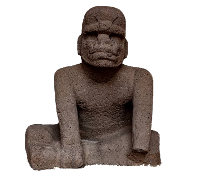
\includegraphics[width=0.5\textwidth]{img/juchiman}
  \apanota{Elaboración propia.}
\end{figure}

\section{Discusión}

[\ldots]

\section{Conclusión}

[\ldots]


\capitulo{Conclusiones y recomendaciones generales}

[\hl{Escriba aquí las conclusiones y recomendaciones generales del trabajo}].


% Referencias en formato APA 7 generadas automáticamente con BibTeX
% \nocite{*} incluye TODAS las referencias del archivo .bib en la lista final
\bibliographystyle{apacite}
\bibliography{referencias}

\end{document}
